\subsubsection{Single point source in arbitrary point}
In the above, we made things simple by assuming that the current source was placed in the origin ${\bf r} = 0$. It is relatively intuitive that if the point source were located in an arbitrary point ${\bf r_1} $, $r$ in the denominator of eq. \ref{eq:pointsource} should be replaced with $|{\bf r-r_1}|}$. To derive this mathematically, we start by noting that the current density integrated over an arbitrary surface containing the source should, as before, be identical to the total source current.

\begin{equation}
\oiint_{S} {\bf i}({\bf r}, t) \cdot  \,d{\bf S} = \oiint_{S} \sigma\nabla\phi({\bf r}, t) \cdot \, d{\bf S}  = I_1
\label{eq:berit1}
\end{equation}

To solve this, it is convenient to chose a spherical surface with radius $R = |{\bf r-r_1}|}$ centered at the source location ${\bf r_1}}$ (Fig. \ref{fig:pointsource}B). We then know that the electrical potential is the same for all ${\bf r}$ in this surface ($\phi({\bf r}, t) = \phi(R,t)$), and that that its gradient is perpendicular to the surface increment. If we use this, eq. \ref{eq:berit1} becomes:

\begin{equation}
4\pi R^2\sigma \frac{d\phi(R)}{dR} = I_1
\label{eq:berit2}
\end{equation}
Integration with respect to $R$ gives us:

\begin{equation}
\phi(R, t) = \phi({\bf r}, t) = \frac{I_1}{4\pi \sigma R} = \frac{I_1}{4\pi \sigma |{\bf r} - {\bf r_1}|}
\label{eq:berit3}
\end{equation}


\begin{equation}
\phi = \frac{I_1}{4\pi \sigma |{\bf r-r_1}|},
\end{equation}

If we have several point-current sources, $I_{1}, I_2, I_3, ... $ in locations ${\bf r_1}, {\bf r_2}, {\bf r_3} ... $), their contributions add up linearly, and the potential in a point ${\bf r}$ is given by:

\begin{equation}
\phi({\bf r}) = \frac{I_1}{4\pi  \sigma {\bf |r-r_1|}} + \frac{I_2}{4\pi  \sigma {\bf |r-r_2|} } + \frac{I_3}{4\pi  \sigma {\bf |r-r_3|} } + ... = \sum_k \frac{I_k}{4\pi  \sigma {\bf |r-r_k|} }.
\label{eq:pointsources}
\end{equation}

\subsection{Current conservation}
Volume conductor theory is essentially based on current conservation in the extracellular medium. Mathematically, current conservation implies that:

\begin{equation}
\nabla {\bf i}({\bf r}, t) = - CSD({\bf r}, t),
\label{eq:CSD1}
\end{equation}
where ${\bf i}$ is the extracellular current density, and $CSD$ is the current source density. Eq. \ref{eq:CSD1} shows that if there are no neuronal current sources, the gradient of the current density must be zero, i.e., $\nabla \cdot {\bf i} = 0$, which tells us that no net current can enter/leave any given point in the extracellular space. The $CSD$ term in Eq. \ref{eq:CSD1} then accounts for  the points where net currents actually do enter or leave the extracellular space in terms of transmembrane neuronal currents.

The current density ${\bf i}$ could in principle include several kinds of electrical currents \cite{Gratiy2017}, but under most conditions ohmic drift currents dominate, and in this chapter we assume that:

\begin{equation}
{\bf i} = \nabla ({\sigma \nabla \phi})
\label{eq:ohmici}
\end{equation}
If we combine Eq. \ref{eq:ohmici} and Eq. \ref{eq:CSD1}, we get:

\begin{equation}
\nabla ({\sigma \nabla \phi}) = - CSD
\label{eq:CSD2}
\end{equation}

If we further assume that the conductivity $\sigma$ is constant, Eq. \ref{eq:CSD2} simplifies to:

\begin{equation}
\sigma \nabla^2 \phi = - CSD
\label{eq:CSD3}
\end{equation}

If we know the $CSD$, we can integrate this expression over space to derive what $\phi$ will be. In principle, the equation can also be used the other way around, i.e., if we record the potential at several points in space, we can use it to predict the underlying current sources. However, this \textit{backward} problem is ill posed, and solutions are not unique \ghn{More on this?}. Here, we focus on the forward modelling problem, i.e., going from a known $CSD$ to a prediction of the extracellular potential. 

\begin{equation}
\nabla^2 \phi = - CSD/\sigma,
\label{eq:trygve}
\end{equation}
where we have introduced the electrical field 

${\bf E}={\bf \nabla} \phi$ \ghn{Comment on this? Maxwell -> quasistatic -> cross-product = 0 implies E is gradient of scalar function. Is anything gained by introducing  {\bf E} at all, when we already have $\phi$? Or how about using {\bf E} instead of $\nabla\phi$ from the start?}, and for now assumed that the conductivity, $\sigma$, is a scalar constant. We integrate each side of this equation over a 3D volume,
\begin{equation}
\iiint_V E({\bf r}) \,d^3V =  - \frac{1}{\sigma} \iiint_V \ CSD({\bf r}) \, d^3V.
\label{eq:trygve2}
\end{equation}
If we consider the simplest possible case of a single point current source $I_1$ in ${\bf r}=0$, the right hand side becomes $-I_1/\sigma$. By Gauss' theorem, we can convert the left hand side to a surface integral, and get:
\begin{equation}
\iiint_V E(r) \,d^3V =  \oiint_{S} E(r) \,d^2S = 4\pi r^2 E(r) = 4\pi r^2 \frac{d\phi}{dr} = -\frac{I_1}{\sigma},
\label{eq:trygve3}
\end{equation}
where we have exploited the spherical symmetry of the problem. Finally, integration with respect to $r$ gives us


\section{PNP og KNP}
Both the PNP formalism and the electroneutral formalism allow us to compute the dynamics of ion concentrations and the electrical potential in the extracellular space of neural tissue containing an arbitrary set of neuronal and glial current sources. For example, in recent work, a version of the electroneutral formalism was developed into a framework for computing the extracellular dynamics (of $c_k$ and $\phi$) in a 3D space surrounding morphologically complex neurons simulated with the NEURON simulation tool \citep{Solbra2018}. However, both the PNP and electroneutral formalisms keep track of the spatial distribution of ion concentrations, and as such they require a suitable meshing of the 3D space, and numerical solutions based on finite difference- or finite element methods. In both cases, simulations can become very heavy, and for systems at a tissue level, the computational demand may become incommensurable. For that reason, there is much to gain from deriving simpler frameworks where effects of ion concentration dynamics are neglected, since, for many scenarios, this may be a good approximation. Below, we will derive these simpler frameworks using the Nernst-Planck fluxes (eq. \ref{eq:JNP}) as a starting point, as this approach will make the involved approximations transparent.

\subsection{General currents in the extracellular space}
Starting more generally, the extracellular current density could in principle have additional contributions from  diffusion of ions, advection and displacement currents: 

\begin{equation}
{\bf i} = {\bf i^{ohm}} + {\bf i^{dif}} + {\bf i^{adv}} + {\bf i^{dis}}, 
\label{eq:generalcurrent}
\end{equation}

The advective current, 
\begin{equation}
{\bf i^{adv}} = F \rho {\bf u}, 
\label{eq:iadv}
\end{equation}
is the current that arises in a bulk solution if the solution has a charge density $\rho$ that it drags along with it due to a bulk flow with velocity ${\bf u}$. 

The displacement current,
\begin{equation}
{\bf i^{dis}} = \frac{\partial \rho}{\partial t},
\label{eq:idis}
\end{equation}
represents the capacitive effect of a medium that allows local charge accumulation, so that $\rho$ can vary with time.  

For the physiological conditions of the extracellular solution, it has been shown theoretically that the charge relaxation time, i.e., the time it takes for $d\rho/dt$ to decay to zero when responding to a change in the electric field, is in the order of 1 ns \cite{Grodzinsky2011, Gratiy2017}. This means that the displacement current (eq. \ref{eq:idis}) will mainly be important under conditions when the electrical field varies with frequencies in the GHz range. As the relevant fields with physiological origin vary with frequencies that are orders of magnitude lower than this, the displacement current can safely be neglected. Related to this, the actual charge accumulation that takes place during a relaxation time of 1 ns is very small. For most practical purposes it is a therefore good approximation to assume that the extracellular medium is electroneutral \cite{Solbra2018}, which means that $\rho = 0$ so that the advective current becomes zero. Hence, for practical purposes, it is safe to assume that both the displacement current (eq. \ref{eq:idis}) and the advective current (eq. \ref{eq:iadv}) give negligible contributions to extracellular dynamics. A more physically rigorous argument for this was given in \cite{Gratiy2017}. 

If we can neglect advective and displacement currents, we are left with the Ohmic drift current and the diffusive current. The Ohmic drift current is given by:
\begin{equation}
{\bf i^{ohm}} = \sigma {\bf E} = - \sigma \nabla \phi,
\label{eq:ohmiciagain}
\end{equation}
where the last equality follows from the quasi-static approximation of Maxwell's equations (Chapter \ref{sec:quasistatic}). In standard VC theory, this is assumed to be the only extracellular current, and we recognize it from eq. \ref{eq:ohmici}. 

Finally, the diffusive current is given by: 
\begin{equation}
{\bf i^{dif}} = -F \sum_k z_k D_k \nabla c_k.
\label{eq:idif}
\end{equation}
It represents the current that arrises when ions (with valence $z_k$ and diffusion constants $D_k$) diffuse along extracellular concentration gradients ($\nabla c_k$), and carry along with them a net charge. Diffusive currents are neglected in standard VC theory under the (\textit{a-priori}) assumption that they are much smaller than Ohmic drift currents at the coarse grained scale of brain tissue. However, the magnitude of diffusive currents depend on the steepness of the concentration gradients in the extracellular solution, and it has been estimated that diffusive will have a notable impact on extracellular potential in physiological conditions with large concentration gradients  \cite{Halnes2016, Gratiy2017}. Diffusive effects on extracellular potentials may therefore be particularly relevant under pathological conditions such as epilepsy, stroke and spreading depression, which are associated with dramatic shifts in local extracellular concentrations (see e.g.,  \cite{Somjen2001, Frohlich2008, Wei2014, Ayata2015}). 

In the reminder of this chapter, we present the theory for extracellular dynamics when the currents in the extracellular space are electrodiffusive, i.e., when the charge carriers in the brain, the ions, move due to diffusion as well as Ohmic drift. 



\subsection{Om CSD}
This the standard expression used in current source density (CSD) theory \citep{Mitzdorf1985, Nicholson1975, Pettersen2006}, where spatially distributed recordings of $\phi$ are used to make theoretical predictions of underlying current sources. When using Eq. \ref{eq:CSDstandard}, it is implicitly assumed that the Laplacian of $\phi$ exclusively reflects transmembrane current sources, and that it is not contributed to by diffusive processes. 



\subsection{\blue{Frameworks for solving the Nernst-Planck equations} }
\label{sec:Eldiff:frameworks}
Let us for now assume that the neuronal source terms $f_k$ are known at all points in space, and that we want to solve the Nernst-Planck continuity equation for the resulting extracellular ion concentration dynamics. If there are $K$ different ion species present in the system of study, eq. \ref{Eldiff:eq:NP} gives us $K$ equations, i.e., one for each individual ion concentrations $c_k$. However, the dynamics of the individual ion species are coupled by the additional variable $\phi$. Hence, we have $K+1$ variables, and are in need of an additional equation for $\phi$. There are two main approaches to this: One can either use the so-called \textit{Poisson-Nernst-Planck (PNP)} framework, or the so-called \textit{electroneutral} framework.

\subsubsection{\blue{The Poisson-Nernst-Planck (PNP) framework}}
The physically most detailed approach for defining $\phi$ in the eq. \ref{Eldiff:eq:NP}) is to use Poisson's equation from electrostatics:
\begin{equation}
\nabla^2 \phi = -\rho/\epsilon.
\label{Eldiff:eq:poisson}
\end{equation}
Here $\epsilon$ is the permittivity of the medium, and the local extracellular charge density $\rho$ is determined from the ionic concentrations: 
\begin{equation}
\rho = F \sum_k z_k c_k.
\label{Eldiff:eq:Frode}
\end{equation}

The system of equations combining Poisson's equation (eq. \ref{Eldiff:eq:poisson}) and the Nernst-Planck equation (eq. \ref{Eldiff:eq:NP})
is called the Poisson-Nernst-Planck (PNP) formalism, and the PNP equations can in principle be solved for arbitrary complex geometries using numerical methods, like the Finite Element Method (FEM). 

To solve the PNP system of equations is extremely computationally demanding. One reason for this is that the concentrations of ions in a given volume of space are almost so that the net positive and negative charges outbalance, so that the medium is very close to electroneutral. A non-zero $\rho$ thus reflects a tiny deviance from electronutrality, and it has been estimated that this deviance typically involves only a fraction $\sim 10^{-9}$ of the ions present \cite{Aguilella1986}. An accurate prediction of $\rho$ from eq. \ref{Eldiff:eq:Frode} thus requires an extreme precision in the modeling of the ionic concentrations $c_k$. Another reason, as we discussed briefly in Section \ref{sec:LJpot}, is that the charge-relaxation time in the extracellular solution, i.e., the time scale that $\rho$ varies on, is in the order of nanoseconds. In addition, any non-zero charge density in neural tissue is predominantly resolved in nano-meter thick layers around neuronal membranes \cite{Grodzinsky2011, Gratiy2017}. Simulations of $\rho$ therefore require a spatiotemporal resolution smaller than nanometers and nanoseconds, and thus a very fine-grained description of the tissue where neuronal, glial and extracellular geometries are explicitly defined.

Due to its computational demand, the PNP framework is not suitable for estimating dynamics at the level of tissue. However, it has been used in neuroscience to study various electrodiffusive processes taking place on a very tiny spatiotemporal scale near and inside membranes \cite{Leonetti1998, Leonetti2004, Lu2007, Lopreore2008, Nanninga2008, Pods2013, Gardner2015}. 


\subsubsection{\blue{The electroneutral framework}}

An alternative to the PNP framework is to replace the Poisson equation (eq. \ref{Eldiff:eq:poisson}) with the simplifying approximation that the bulk solution is electroneutral:
\begin{equation}
\alpha F \sum_k z_k c_k = 0.
\label{Eldiff:eq:electroneutral}
\end{equation}
Eq. \ref{Eldiff:eq:electroneutral} is then imposed as a constraint when solving eq. \ref{Eldiff:eq:NP} by use of some numerical method. When using this approach, the constraint determines the value that $\phi$ must have for there to be no charge accumulation anywhere in the extracellular space, a problem which has a unique solution. To use our previous cartoon example as a reference, the electroneutral scheme circumvents nanosecond-fast charge relaxation process (Fig. \ref{Eldiff:fig:diffpot}B) by assuming that the system is always in quasi-steady (Fig. \ref{Eldiff:fig:diffpot}C). It has been shown that this is a good approximation on spatiotemporal scales larger than micrometers and microseconds \citep{Grodzinsky2011, Pods2017, Solbra2018}, and that this approximation gives stable solutions with an arbitrary coarse resolution.

In practice, it is often more convenient to impose the electroneutrality constraint on differential form:
\begin{equation}
\alpha F \sum_k{z_k \frac{\partial c_k}{\partial t}} = 0.
\label{Eldiff:eq:electroneutral2}
\end{equation}

We note that the electroneutrality constraint (eq. \ref{Eldiff:eq:electroneutral} or \ref{Eldiff:eq:electroneutral2}) only applies to the bulk solution, i.e. to points in extracellular space (or intracellular space, if one were to use such a formalism inside neurons) where there is no membrane current source. The membrane dynamics must then be dealt with separately. In previous implementations, this problem has been tackled in various ways, depending on whether the framework was tailored to simulate intracellular dynamics, extracellular dynamics, or both, and whether it was tailored for applications to a coarse grained (tissue level) spatial scale or a more microscopic scale \citep{Qian1989, Mori2008, Mori2009, Mori2009a, Mori2011, Halnes2015, Halnes2013, Pods2017, Niederer2013, OConnell2016, Solbra2018, tuttle2019, ellingsrud2020}. We shall revisit some of these frameworks in Chapter \ref{sec:Schemes}. In this Section, we will only introduce one of them, the so-called Kirchhoff-Nernst-Planck (KNP) framework, since this was tailored to compute extracellular dynamics on the coarse-grained scale that we have focused on in this chapter \citep{Solbra2018}.


\subsubsection{\blue{The electroneutral Kirchhoff-Nernst-Planck framework}}
The KNP framework, in the form presented in \cite{Solbra2018}, focuses solely on the dynamics in the extracellular space, when "receiving" input from discrete neuronal sources. In this sense it is similar to standard VC theory, except that it includes the dynamics of ion concentrations and their effects on extracellular potentials. Unlike standard VC theory, where the different kinds of transmembrane currents, such as leakage currents, capacitive currents, and ion specific active currents, can be grouped into a single source variable $C$ for the total CSD at each segment, the KNP scheme requires the sources to be expressed as a set of ion specific flux-sources, i.e., one source $f_k$ per ion species $k$ (in eq. \ref{Eldiff:eq:NP}), and an additional capacitive neuronal membrane current source density, $C_{cap}$, the only source term not accounted for in the set $f_k$.

In the KNP-framework, membrane dynamics is accounted for by replacing the electroneutrality constraint (eq. \ref{Eldiff:eq:electroneutral2}) with
\begin{equation}
\alpha F \sum_k{z_k \frac{\partial c_k}{\partial t}} = C_{cap},
\label{Eldiff:eq:electroneutral3}
\end{equation}
where 
\begin{equation}
C_{cap} = {\alpha}\frac{\partial \rho_{mem}}{\partial dt},
\label{Eldiff:eq:Andreas}
\end{equation}
reflects the membrane potential dynamics of a neuron. As $C_{cap}$ is zero at locations where there is no neuronal membrane source, eq. \ref{Eldiff:eq:electroneutral2} still holds in the bulk solution. 

The constraint in eq. \ref{Eldiff:eq:electroneutral3} was essentially what we used earlier to get from eq. \ref{Eldiff:eq:chargecontinuity} to eq. \ref{Eldiff:eq:eldiffCSD2}. The KNP scheme thus uses Eq. \ref{Eldiff:eq:eldiffCSD2} with $C$ as defined in eq.  \ref{Eldiff:eq:CSDdecomposed} to to derive $\phi$:
\begin{equation}
\nabla \cdot (\sigma\nabla\phi) = - F \sum_k z_k f_k -  C_{cap} - F\alpha \nabla \cdot \left (\sum_k{z_k \tilde{D_k}{\bf \nabla} c_{k}} \right).
\label{Eldiff:eq:KNPfinal}
\end{equation}
Through this equation, $\phi$ is uniquely determined by the ion concentrations ($c_k$) and the neuronal CSD, the latter represented by the first two terms on the right hand side.

Since the KNP equations are coupled in the sense that $\phi$ affects the dynamics of $c_k$ and $c_k$ the dynamics of $\phi$, the KNP set of equations do not give any simple analytical relationship between the neuronal CSD and the extracellular potential. Instead, the KNP set of equations must be solved on some numerical framework using a suitable meshing of the tissue volume, i.e., like that depicted in Fig. \ref{Eldiff:fig:KNPmesh}.

\begin{figure}[!ht]
\begin{center}
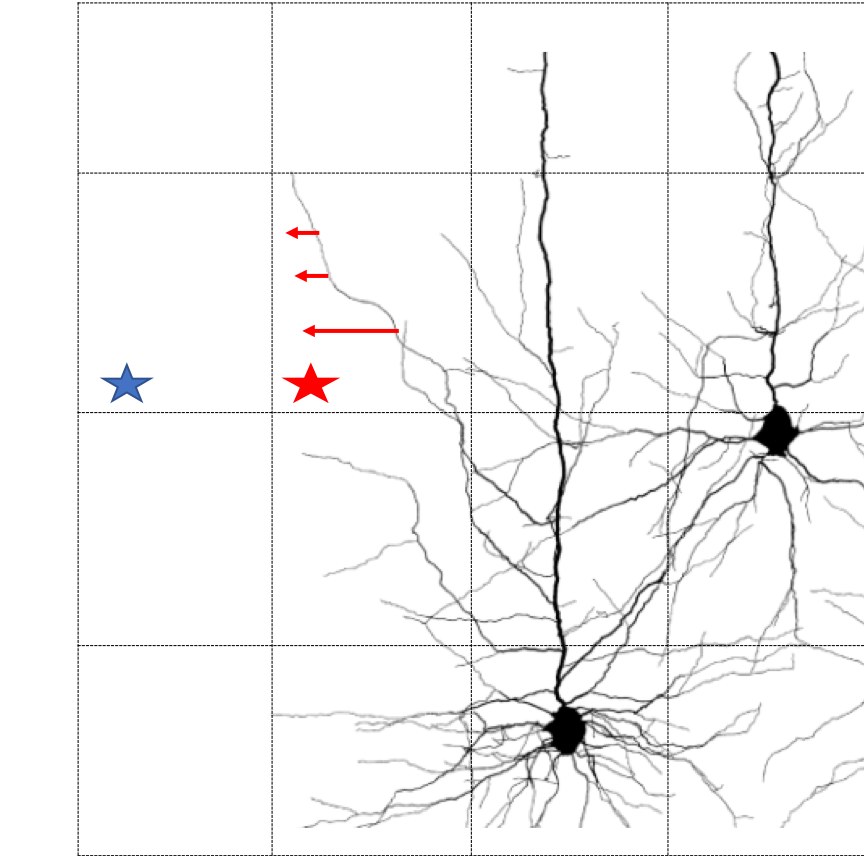
\includegraphics[width=0.5\textwidth]{Figures/Eldiff/KNP.png}
\end{center}
\caption{\textbf{KNP scheme}. Blue star: Mesh cell containing no neuronal sources, so that $C=0$. Red star: Mesh cell containing neural sources. Here $C$ can be computed by summing over all neuronal transmembrane currents, including the capacitive current, and dividing by the volume of the mesh cell. \ghnote{LAGE LITT MER INFORMATIV FIG HER OM VI SKAL HA FIG HER.}}
\label{Eldiff:fig:KNPmesh}
\end{figure}


\section{UTKLIPP FRA SCHEMES}
These ephaptic effects may include the effect that the extracellular potential, and, if accounted for, variations in extracellular ionic concentrations, have on the neurodynamics. Changes in extracellular ion concentrations may also give rise to extracellular diffusion potentials, as we explored in (Chapter \ref{sec:Eldiff}).


and, also the effect of extracellular concentration changes  (if included in the model) on ionic reversal potentials (Eq. \ref{Neuron:eq:revpots}). 


A key parameter, and sometimes variable, in VC theory is the conductivity ($\sigma$) of the extracellular medium. In Chapter \ref{sec:Sigma} we give an overview of the experimental and theoretical estimates of $\sigma$. 


In previous implementations, this problem has been tackled in various ways, depending on whether the framework was tailored to simulate intracellular dynamics, extracellular dynamics, or both, and whether it was tailored for applications to a coarse grained (tissue level) spatial scale or a more microscopic scale \citep{Qian1989, Mori2008, Mori2009, Mori2009a, Mori2011, Halnes2015, Halnes2013, Pods2017, Niederer2013, OConnell2016, Solbra2018, tuttle2019, ellingsrud2020}.



Another assumption that is typically used when applying VC theory is that the extracellular potential $\phi$ does not have any (ephaptic) effect on the neuronal membrane potential dynamics. This simplifies computations dramatically, because it allows us to perform them in a two-step procedure where we (i) first compute the neurodynamics independently, typically under the assumption that the extracellular potential is zero ($\phi = 0$), and (ii) next use the analytical VC-expression to compute a nonzero $\phi$. The motivation for using this evidently inconsistent approach is that $\phi$ is typically so much smaller than the membrane potential that the ephaptic effects can be neglected without any severe loss in accuracy. This might not be true for all biologically relevant geometries and scenarios, and frameworks that compute the extracellular, membrane and intracellular potentials in a self consistent manner exist (all arrows in Fig. \ref{Intro:fig:Knallfigur}C), as do unified frameworks that compute both ion concentrations and electrical potentials in a self consistent manner (all arrows in Fig. \ref{Intro:fig:Knallfigur}D). A summary of available frameworks for computing extracellular potentials (and ion concentrations) is given in Chapter \ref{sec:Schemes}.

We note that there are two commonly used conventions for defining the variables and parameters involved in computing extracellular dynamics. One can either define them relative to (i) the unit volume and unit cross section area of the tissue as a whole, or (ii) relative to to the unit volume and unit cross section area of the fraction of it that is extracellular. The first (i) of these conventions is standard in VC theory (Chapter \ref{sec:VC}), whereas the second (ii) is more common in electrodiffusive models. In this book, we have chosen to use the same convention (i) for both VC theory and electrodiffusive theory, since it will make it easier to compare the two directly. However, we made one exception, and defined $c_k$ using the extracellular fraction of the tissue volume as reference. The advantage of using this alternative reference volume for $c_k$ is that $c_k$ then represents a "real" extracellular concentration (as it is measured). The disadvantage is that the volume fraction $\alpha$ will appear in the continuity equation, something that we could have avoided by using convention (i) also for $c_k$. However, we thought that we could live with that.



To solve this set of equations (one instance of eq. \ref{Eldiff:eq:NPe} for each ion species $k$), we need an additional constraint for the additional variable $\phi$. For this, we use the assumption that the bulk solution should be electroneutral, but do account for charge accumulation at neural membranes (cf. eq. \refl{Schemes:eq:rhocap}). In the HHC+ED framework, this constraint is expressed as:
\begin{equation}
F \sum_k{z_k \frac{\partial c_k}{\partial t}} = C_e^{cap},
\label{Schemes:eq:electroneutral3}
\end{equation}
where the (neural) capacitive current source density:
\begin{equation}
C_e^{cap} = {\alpha}\frac{\partial \rho_e^{mem}}{\partial dt},
\label{Schemes:eq:Andreas}
\end{equation}
reflects the membrane potential dynamics of a neuron due to charge accumulating on the external membrane surface. As $C_e^{cap}$ is zero at all locations where there is no neuronal membrane source, the bulk solution of the extracellular space will be electroneutral.


The scheme (S1) used by Mori and Peskin \citep{Mori2006, Mori2009}, also used by Pods \citep{Pods2017}, was based on introducing additional state variables for the ion concentrations building up the membrane charge. 


were defined to keep track of the ions building up the charge stored inside the membrane Debye layer. The membrane concentrations were then derived as a function of the concentration profile immediately outside the membrane, and constrained so that it they summed up to the correct membrane charge density (\eta_{mr} in eq. \ref{Schemes:eq:rhocap}).

In the scheme (S2) used by Ellingsrud et al. \citep{ellingsrud2020} which they there referred to as the Kirchhoff-Nernst-Planck + Extracellular-Membrane-Intracellular (KNP-EMI) scheme, the membrane boundary condition was instead based on letting $i_{cap}$ in eq. \ref{Schemes:eq:rhocapt} be defined so that the contributions ($i^k_{cap}$) from the various ion species $k$ were of the same ratio as their concentrations $c_k^r$ in the bulk solution close to the membrane at either side. The membrane charge was not introduced as additional state variables, but represented as a nonzero charge accumulation in the bulk solution immediately inside and outside the membrane. 


\item In the approach (A2) by Ellingsrud et al. \citep{ellingsrud2020}, which they there referred to as the Kirchhoff-Nernst-Planck + Extracellular-Membrane-Intracellular (KNP-EMI) scheme, the membrane boundary condition was instead based on (i) using the differential form of eq. \ref{Schemes:eq:rhocap}:
\begin{equation}
I_{cap}^r = \pm \frac{\partial \rho_{m}^r}{\partial dt}, 
\label{Schemes:eq:rhocap2}
\end{equation}
where the left hand side followed from the definition of the capacitive membrane current (cf. eq. \ref{Neuron:eq:HHcap}). $I_{cap}$, which is given by the membrane potential dynamics computed with the a HH-type framework, was then (ii) made ion specific, and defined so that the ratio between the contributions ($I^k_{cap}$) from the various ion species $k$ was identical to the ratio between the various species $c_k^r$ in the bulk solution close to the membrane at either side.
\end{itemize}





To solve this set of equations (one instance of eq. \ref{Eldiff:eq:NPe} for each ion species $k$), we need an additional constraint for the additional variable $\phi$. For this, we use the assumption that the bulk solution should be electroneutral, but do account for charge accumulation at neural membranes (cf. eq. \refl{Schemes:eq:rhocapt}). In the HHC+KNP scheme, this constraint is expressed as:
\begin{equation}
F \sum_k{z_k \frac{\partial c_k}{\partial t}} = f_{cap},
\label{Schemes:eq:electroneutral3}
\end{equation}
where the (neural) capacitive current source density:
\begin{equation}
f_{cap} = \frac{\partial \rho_e^{mem}}{\partial dt},
\label{Schemes:eq:Andreas}
\end{equation}
reflects the membrane potential dynamics of a neuron due to charge accumulating on the external membrane surface. Eq. \ref{Schemes:eq:Andreas} is the same as eq. \ref{Schemes:eq:rhocapt}, but with extracellular surface charge density $\eta_e^{mem}$ (C/m$^2$) converted to a volume charge density, $ \rho_e^{mem}$ (C/m$^3$), defined as the total extracellular membrane charge within a piece of tissue, divided by extracellular volume in this piece of tissue. As $f_{cap}$ is zero at all locations where there is no neuronal membrane source, the bulk solution of the extracellular space will be electroneutral.

\subsubsection{\blue{Kirchhoff-Nernst-Planck framework for extracellular electrodiffusion}}

The constraint in eq. \ref{Schemes:eq:electroneutral3} was essentially what we used in Chapter \ref{sec:Eldiff} to get from eq. \ref{Eldiff:eq:chargecontinuity} to eq. \ref{Eldiff:eq:eldiffCSD2}. The KNP scheme thus uses Eq. \ref{Eldiff:eq:eldiffCSD2} with $C$ as defined in eq.  \ref{Eldiff:eq:CSDdecomposed} to to derive $\phi$:
\begin{equation}
\nabla \cdot (\sigma\nabla\phi) = - F \sum_k z_k f_k -  C_{cap} - F\alpha \nabla \cdot \left (\sum_k{z_k \tilde{D_k}{\bf \nabla} c_{k}} \right).
\label{Schemes:eq:KNPfinal}
\end{equation}
Through this equation, $\phi$ is uniquely determined by the ion concentrations ($c_k$) and the neuronal CSD, and with that, the Nernst-Planck equations (eq. \ref{Schemes:eq:NPe}) can be solved on a suitable numerical framework.


\begin{equation}
\frac{\partial c_k}{\partial t} = {\bf \nabla} \cdot \left[ \tilde{D}_k {\bf \nabla} c_k + \frac{\tilde{D}_k z_k c_k}{\psi} {\bf \nabla} \phi \right] + f_k, 
\label{Schemes:eq:NPe}
\end{equation}
where $\tilde{D}_k$ denotes the effective extracellular diffusion constant for an ion species $k$. This equation can be solved when combined with an electroneutrality constraint such as that in the 
eq. \ref{Schemes:eq:electroneutral2} for the bulk solution and eq. \ref{Schemes:eq:rhocapt} at the membrane. 
\end{itemize}



\ghnote{Maybe make this a box?}
\begin{floatingbox}[h]
\caption{Hodgkin-Huxley model}
\begin{equation}
c_m \frac{dV_m}{dt} = -\bar{g}_L(V_m-E_L) - \bar{g}_{Na} m^3 h (V_m - E_{Na}) - \bar{g}_{K} n^4 (V_m - E_{K}).
\label{Neuron:eq:HHfull}
\end{equation}
\begin{equation}
\frac{dx(V_m,t)}{dt} = \frac{x_{\infty}(V_m) - x}{\tau_x(V_m)},  \, \text{for } x = \{m,h,n\}.
\label{Neuron:eq:HHgates}
\end{equation}

\begin{table}[h!]
    \caption{\textbf{The Hodgkin-Huxley model.}}
    \label{Neuron:tab:HH}
\begin{center}
    \begin{tabular}{l}
    \hline
    $x_{\infty}(V_m) = \frac{\alpha_x(V_m)}{\alpha_x(V_m) + \beta_x(V_m)}$ for $x = m,n,h$ \\ \hline
    $ \alpha_n = \frac{0.01 \mathrm{ms}^{-1} V_m+55 \mathrm{mV}}{1-e^{-(V_m+55 \mathrm{mV})/10 \mathrm{mV}}}$  \\ \hline
    $ \beta_n = 0.125 \mathrm{ms}^-1 e^{-(V_m+65 \mathrm{mV})/80 \mathrm{mV}} $  \\ \hline
    $ \alpha_m = \frac{0.1 \mathrm{ms}^{-1} V_m+ 40 \mathrm{mV}} {1-e^{-(V_m+40 \mathrm{mV})/10 \mathrm{mV}}}$  \\ \hline
    $\beta_m = 4 \mathrm{ms}^{-1} e^{-(V_m+65  \mathrm{mV})/18 \mathrm{mV}} $  \\ \hline
    $\alpha_h = 0.07 \mathrm{ms}^{-1} e^{-(V_m+65 \mathrm{mV})/20 \mathrm{mV}}$  \\ \hline
    $\beta_h = \frac{1 \mathrm{ms}^{-1}}{1+e^{-(V_m+35 \mathrm{mV}))/10 \mathrm{mV})}} $  \\ \hline
    $c_m = 1.0 \mu $F/cm$^2$ \\ \hline
    $\bar{g}{Na} = 120\times 10^{-9}$ m$^2$/s\\ \hline
    $\bar{g}_{K} = 36$ mS/cm$^2$ \\ \hline
    $\bar{g}_{L} = 0.3$ mS/cm$^2$ \\ \hline
    $E_{Na} = 50$ mV \\ \hline
    $E_{K} = -77$ mV \\ \hline
    $E_{L} = -54.4$ mV \\ \hline
    \end{tabular}
    \end{center}
\end{table}

\begin{figure}[h!]
\begin{center}
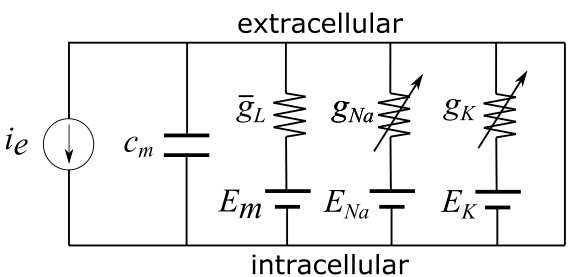
\includegraphics[width=0.8\textwidth]{Figures/Neuron/HHmodel.png}
\end{center}
\caption{\textbf{Hodgkin Huxley model.}}
\label{Neuron:fig:HHcircuit}
\end{figure}
\label{box:Neuron:HH}
\end{floatingbox}


\subsection{\orange{GH: Temporal solutions of cable equation}}
\label{sec:Neuron:cabletemp}
In Fig. \ref{Neuron:fig:Semiinf}A we simulated numerically the response of a cylindrical neuron to a  synaptic input in one end. It is possible to derive some analytical results also for the temporal solution of $V$ in a passive cable is \cite**{rall1969}:
\begin{equation}
V(x,t) = C_0(x) e^{-t/\tau_0} + C_1(x) e^{-t/\tau_1} + C_2(x) e^{-t/\tau_2} + \ldots, 
\label{Neuron:eq:cabletemporal}
\end{equation}
where the coefficients $C_n(x)$ depend on the distance along the cable, while $\tau_0 = \tau_m = R_m C_m$ is the \emph{membrane time constant} (eq. \ref{Neuron:eq:timeconst}), and the other time constants have successively smaller values ($\tau_0 > \tau_1 > \tau_2 > \ldots$). 


The simulation showed that the synaptic input lead to a peak response in $V$ that was smaller in amplitude and arrived later the further away from the injection site


 However, the potential is about the same at all points along the cable a few milliseconds after the stimulus was delivered. After this, $V$  decays. 
 This decay takes place at the slower time scale of the membrane time constant, which in this simulation was 10~ms ($R_m=10\,\text{k}\Omega \text{cm}^2$, and $c_m=1\,\mu\text{F}/\text{cm}^2$). 





\section{Quasistatic}


\subsection{\orange{GH: Debye screening}}
The Coulomb force (eq. \ref{eq:Basics:CoulombF}) causes positive charges to attract negative charges and repel other positive charges. An effect of this is that positive charges in a conductive medium will tend to surround themselves with negative charges, and vice versa. Consequently, the numbers of positive and negative charges in a finite volume of space tends to be in balance, and any finite reference volume of brain tissue will, on the coarse-grained scale, be practically electroneutral \cite**{Nunez2006,Grodzinsky2011}. If this were not the case, and a volume did contain a net charge density $\rho$, the very strong Coulomb-forces associated with it would cause $\rho$ to decay to zero at a rate proportional to the so-called \textit{charge-relaxation time}, which in brain tissue is in the order of a nanosecond \cite**{Grodzinsky2011}. 

Related to this, the Coulomb force also gives rise to a phenomenon called Debye screening, 

The closely balanced negative and positive charges will tend to shield (cancel out) the electric fields from one another, so that neither of them give any contribution to the field measured at some distance away from the charges. 




Of course, a non-zero electric field or potential does require some charge separation somewhere. In the brain, this predominantly happens at the capacitive neuronal membranes, and then on a very small spatial scale. As we described earlier, a patch of membrane has the capacity to separate a charge $q$ on the interior side from a charge $-q$ on the exterior side. However, since the membrane is just some nanometers thick, the two charges $-q$ and $q$ are very close in space, and will shield each others' contributions to extracellular fields measured at some distance from the membrane. 

The practical implication of electroneutrality and shielding effects is that, when we study extracellular potentials (or fields), we can neglect contributions from any particular distribution of charges, and instead compute extracellular potentials from the constraint that there should be no charge accumulation anywhere in the extracellular space. 




\subsection{\blue{Extracellular currents are exclusively due to electric drift}}
\label{sec:Basics:onlyohmic}
When analyzing extracellular currents in the brain, it is common to assume that they are purely due to electric drift, as we do when using the volume conductor (VC) theory that we present in \Fref{chap:VC}. In principle, a current could have additional contributions from ionic diffusion, advection currents, capacitive (displacement) currents, and electromagnetic induction, so that the total current density would be:
\begin{equation}
{\bf i} = {\bf i}_\text{ohm} + {\bf i}_\text{diff} + {\bf i}_\text{adv} + {\bf i}_\text{cap} + {\bf i}_\text{ind},
\label{VC:eq:generalcurrent}
\end{equation}

As the capacitive current is proportional to $\partial {\bf E}/\partial t$, and the inductive currents is proportional to $\partial {\bf B}/\partial t$, it follows from the quasi-magnetostatic and quasi-electrostatic approximations, respectively, that they are zero in the extracellular medium.

An advective current\index{Advective current},
\begin{equation}
{\bf i}_\text{adv} = F \rho {\bf u},
\label{VC:eq:iadv}
\end{equation}
arises in a bulk solution if the solution has a charge density $\rho$ that it drags along with it due to a bulk flow with velocity ${\bf u}$. As we argued in \fref{sec:Basics:Debye}, the extracellular medium is practically electroneutral ($\rho \simeq 0$), and the advective current therefore becomes negligible. A more thorough argument for this was given in \citeasnoun**{Gratiy2017}.

The diffusive current\index{Diffusive current},
\begin{equation}
{\bf i}_\text{diff} = -F \sum_k z_k D_k {\bf \nabla} c_k,
\label{VC:eq:idif}
\end{equation}
arises when ions (with valence $z_k$ and diffusion constants $D_k$) diffuse along concentration gradients (${\bf \nabla} c_k$), and carry with them a net charge. It has been suggested that diffusive currents can have a notable impact on $\phi$ in physiological conditions with large concentration gradients \cite**{Halnes2016}, especially if ion concentration gradients vary quite rapidly with time \cite**{Gratiy2017}. Diffusive effects on $\phi$ may therefore be particularly relevant under pathological conditions such as epilepsy, stroke and spreading depression, which are associated with dramatic shifts in local extracellular concentrations (see e.g.,  \cite**{Somjen2001,Frohlich2008,Wei2014,Ayata2015}).

To account for diffusive effects, one needs to compute not only the electrical potential, but also the ion concentration dynamics of all involved ions at all points in space. This can not \gen{Da jeg var liten mener jeg at vi maatte skrive "cannot" paa skolen, men det var kanskje et fenomen lokalt baade i tid og rom?} be done using VC theory in the standard form presented in \Fref{chap:VC}, but can be done using Finite Element Methods (see e.g., \cite**{Solbra2018}). We go through the theory for modeling electrodiffusive systems in \fref{sec:Eldiff}.

Under normal conditions, drift currents are likely to have a much bigger impact on the time course of $\phi$ than diffusive currents. Standard VC theory, which neglects diffusive effects, will likely make quite good predictions of $\phi$ under most experimental conditions \cite**{Halnes2016,Gratiy2017}.





